\documentclass[12pt, a4paper, oneside]{ctexart}
\usepackage{amsmath, amsthm, amssymb, appendix, bm, graphicx, mathrsfs, geometry, xcolor, subcaption, float, fancyhdr}
\geometry{left=2.54cm, right=2.54cm, top=3.18cm, bottom=3.18cm}
\usepackage[colorlinks, linkcolor=black]{hyperref}

\usepackage{listings}		% 为了避免与页眉的兼容问题可将listings放入table环境中
\lstset{
    basicstyle          =   \sffamily,          % 基本代码风格
    keywordstyle        =   \color{blue},          % 关键字风格
    keywordstyle    =   [2] \color{teal},
    commentstyle        =   \rmfamily\itshape,  % 注释的风格,斜体
    stringstyle         =   \ttfamily,  % 字符串风格
    flexiblecolumns,                % 别问为什么,加上这个
    numbers             =   left,   % 行号的位置在左边
    showspaces          =   false,  % 是否显示空格,显示了有点乱,所以不现实了
    numberstyle         =   \zihao{-5}\ttfamily,    % 行号的样式,小五号,tt等宽字体
    showstringspaces    =   false,
    captionpos          =   t,      % 这段代码的名字所呈现的位置,t指的是top上面
    frame               =   lrtb,   % 显示边框
    basicstyle          =   \zihao{-4}\ttfamily,
    stringstyle         =   \color{magenta},
    commentstyle        =   \color{red}\ttfamily,
    breaklines          =   true,   % 自动换行,建议不要写太长的行
    columns             =   fixed,  % 如果不加这一句,字间距就不固定,很丑,必须加
    basewidth           =   0.5em,
}
\pagestyle{fancy}
\lhead{\textit{\leftmark}}
\chead{} 
\rhead{\textit{\rightmark}}
\lfoot{} 
\cfoot{\thepage}
\rfoot{}
\renewcommand\headrulewidth {0pt} 

\linespread{1.5}
\renewcommand{\abstractname}{\Large\textbf{摘要}}

\begin{document}

\thispagestyle{empty}

\begin{figure}[t]
    \centering
    
\includegraphics[width=13cm]{../pic/xjtu.png}
\end{figure}

\vspace*{\fill}
    \begin{center}
        \centering
        \vspace{-3cm}
        \fangsong\huge{本科生课程报告} \\\kaishu \Huge{\textbf{基于Java事件处理机制的\\RBAC0权限模型实现}}
    \end{center}
\vspace*{\fill}

\begin{table}[b]
    \centering
    \large
    \begin{tabular}{ll}
        \textbf{课程:} & 软件系统设计与分析 \\
        \textbf{姓名:} & 杨豪 \\
        \textbf{班级:} & 软件2101 \\
        \textbf{时间:} & 2022年10月 \\
    \end{tabular}
\end{table}

\newpage

\thispagestyle{empty}
\begin{abstract}
    在Java语言中,当用户与GUI组件交互时,GUI组件能够激发一个相应事件。例如,用户按动按钮、滚动文本、移动鼠标或按下按键等,都将产生一个相应的事件。
    Java提供完善的事件处理机制,能够监听事件,识别事件源,并完成事件处理。RBAC模型即基于角色的访问控制,是一种很有效的权限分配模型。本文从RBAC模型簇中最基本的模型RBAC0的概念开始,
    介绍了用PowerDesigner设计RBAC0并将其和Java的事件处理机制联系的实现方法。
    最后比较并分析了RBAC模型簇内常见模型的特点。
    \par\textbf{关键词:}事件处理机制; RBAC. 
\end{abstract}

\newpage
\pagenumbering{Roman}
\setcounter{page}{1}
\thispagestyle{plain}
\tableofcontents
\newpage
\setcounter{page}{1}
\pagenumbering{arabic}

\section{RBAC0模型概述}

\subsection{RBAC模型思想}

RBAC(Role-Based Access Control)是基于角色的访问控制。在RBAC中,权限与角色相关联,
而用户通过成为适当角色的成员而得到这些角色的权限,这就极大地简化了权限的管理。
这样管理都是层级相互依赖的,权限赋予给角色,而把角色又赋予用户,这样的权限设计很清楚,管理起来很方便。

虽然可以直接给用户分配权限,只是直接给用户分配权限,少了一层关系,扩展性弱了许多,适合那些用户数量、角色类型少的平台。
对于通常的系统,比如:存在多个用户拥有相同的权限,在分配的时候就要分别为这几个用户指定相同的权限,修改时也要为这
几个用户的权限进行一一修改。有了角色后,我们只需要为该角色制定好权限后,将相同权限的用户都指定为同一个角色即可,便于权限管理。
对于批量的用户权限调整,只需调整用户关联的角色权限,无需对每一个用户都进行权限调整,既大幅提升权限调整的效率,又降低了漏调权限的概率。

\subsection{RBAC0模型}

RBAC模型可以分为:RBAC0、RBAC1、RBAC2、RBAC3四种。其中RBAC0是基础,也是核心的底层逻辑,RBAC1、RBAC2、RBAC3都是以RBAC0为基础的升级。

\begin{figure}[H]
    \centering
    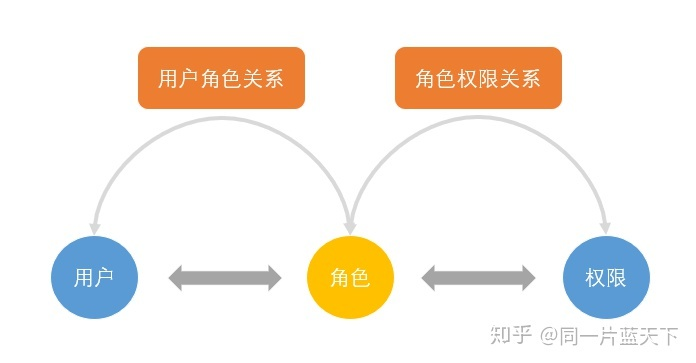
\includegraphics[width = 1\textwidth]{../pic/1/1.2.jpg}
    \caption{RBAC0模型思路}
\end{figure}

\begin{figure}[H]
    \centering
    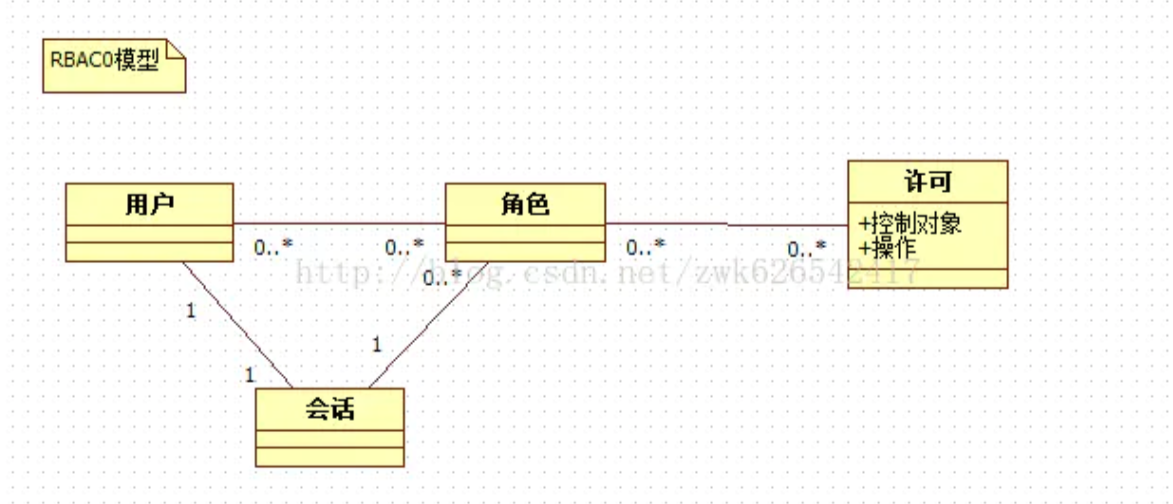
\includegraphics[width = 1\textwidth]{../pic/1/1.1.png}
    \caption{RBAC0数据库表图}
\end{figure}


\section{RBAC0模型的实现}

下面具体讲述如何将Java中的Action事件处理机制和RBAC0模型相结合并实现,此处参考西安交通大学教务平台的成绩
公布系统设计了一个大学生成绩公布系统,并实现了RBAC0模型的权限控制方法。

\subsection{数据库的建立}

参照RBAC0模型的概念,利用PowerDesigner设计得到概念模型UML图如下

\begin{figure}[H]
    \centering
    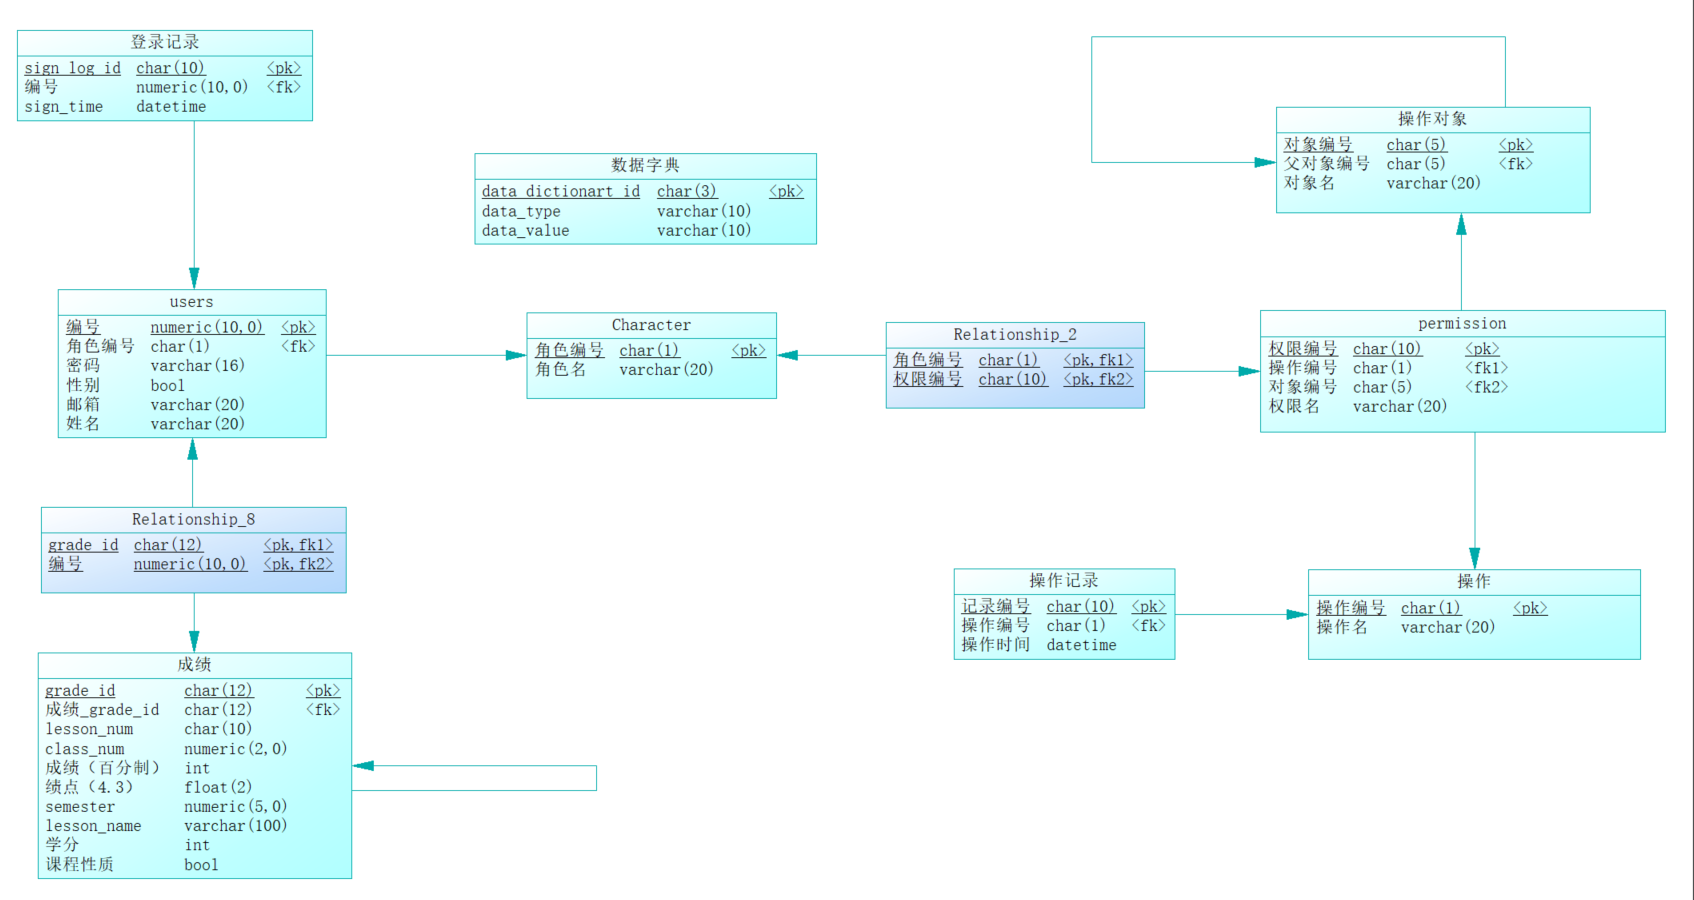
\includegraphics[width = 1\textwidth]{../pic/2/2.1.png}
    \caption{基于RBAC0的学生成绩管理系统的概念模型}
\end{figure}

通过PowerDesigner内置的工具转换物理模型如下

\begin{figure}[H]
    \centering
    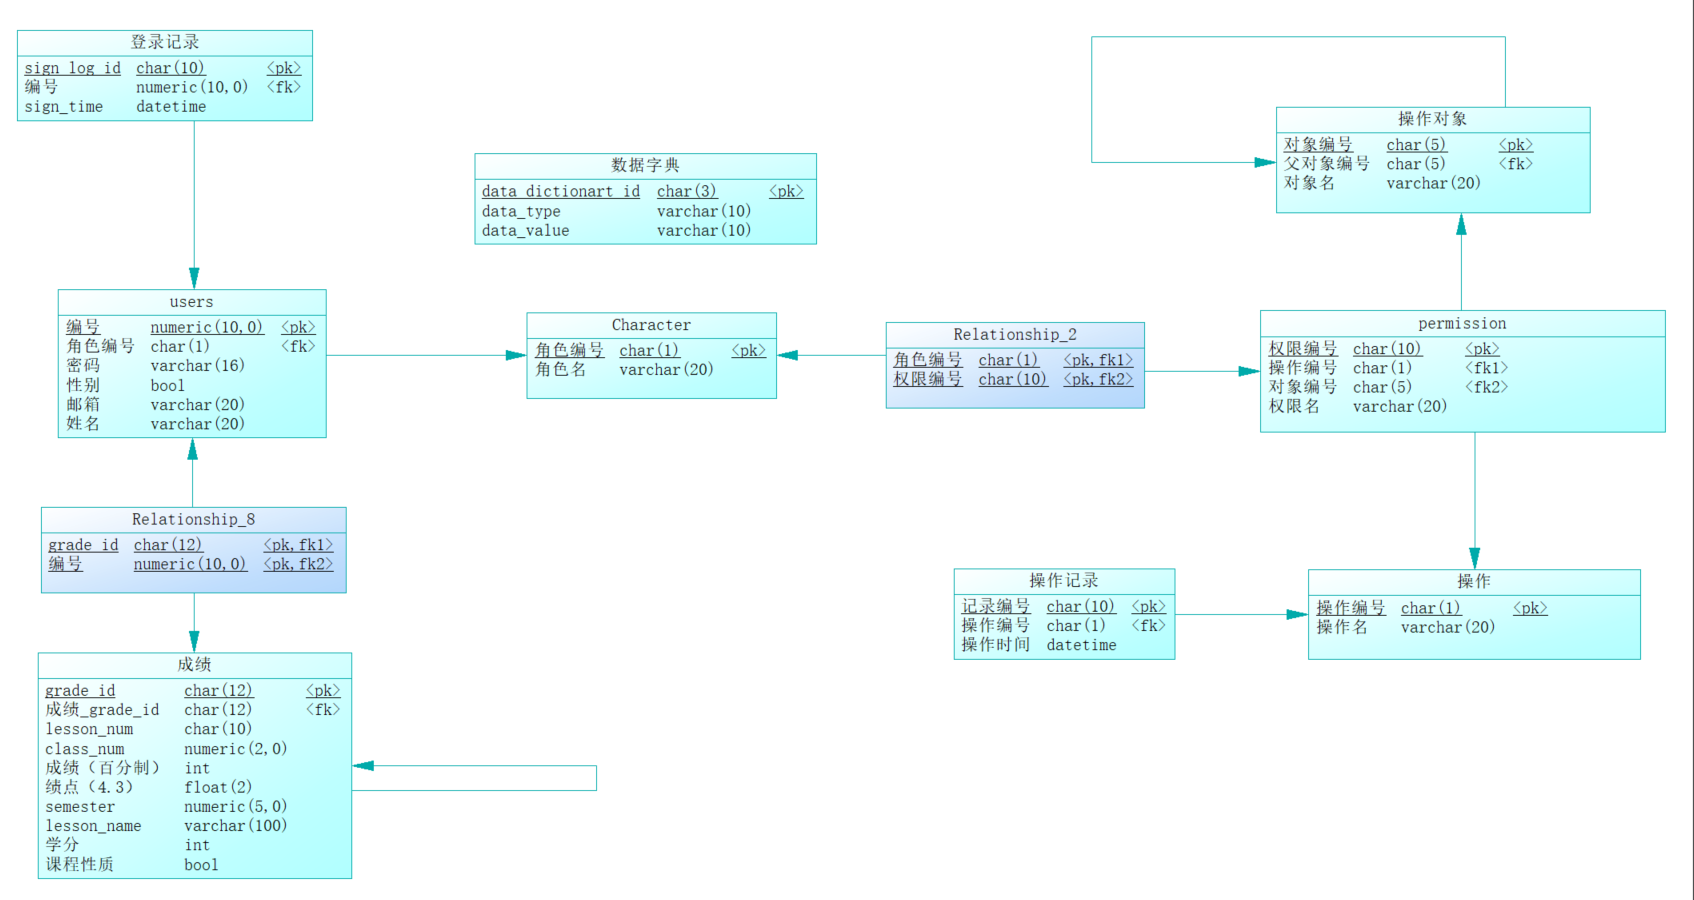
\includegraphics[width = 1\textwidth]{../pic/2/2.1.png}
    \caption{基于RBAC0的学生成绩管理系统的物理模型}
\end{figure}

并通过PowerDesigner内置的工具转换得到sql代码。

\subsection{GUI的搭建}

因为任务要求使用Action事件处理机制,所以首先需要用JavaSwing搭建一个GUI。

\begin{figure}[H]
    \centering
    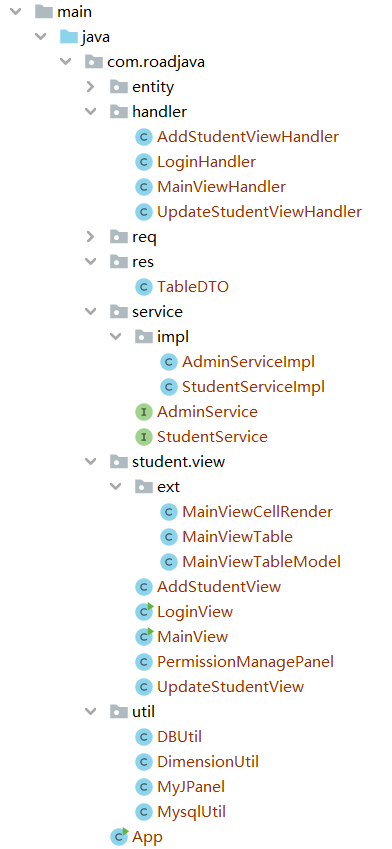
\includegraphics[width = 0.4\textwidth]{../pic/all.png}
    \caption{初始登陆界面}
\end{figure}


\begin{figure}[H]
    \centering
    
\includegraphics[width = 0.7\textwidth]{../pic/3/3.0.png}
    \caption{初始登陆界面}
\end{figure}

\begin{figure}[H]
    \centering
    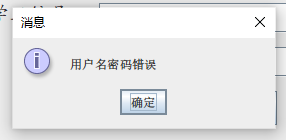
\includegraphics[width = 0.5\textwidth]{../pic/3/3.1.png}
    \caption{输入空}
\end{figure}

\begin{figure}[H]
    \centering
    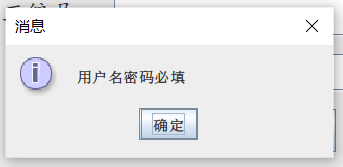
\includegraphics[width = 0.5\textwidth]{../pic/3/3.2.png}
    \caption{密码错误}
\end{figure}

\begin{figure}[H]
    \centering
    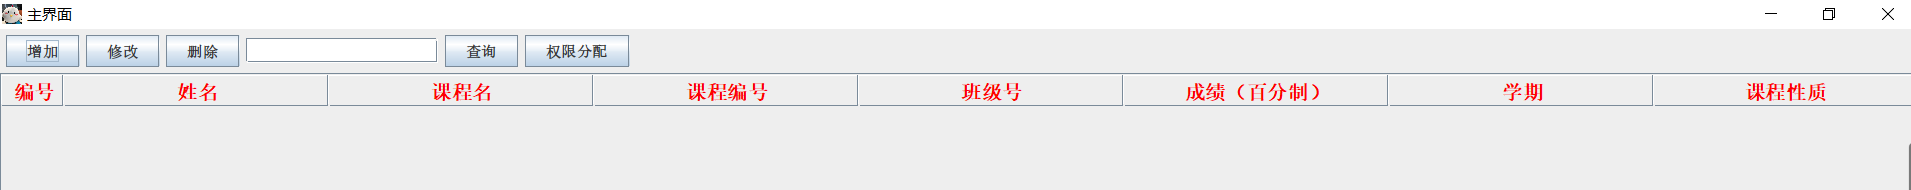
\includegraphics[width = 1\textwidth]{../pic/3/3.3.png}
    \caption{主界面}
\end{figure}

\begin{figure}[H]
    \centering
    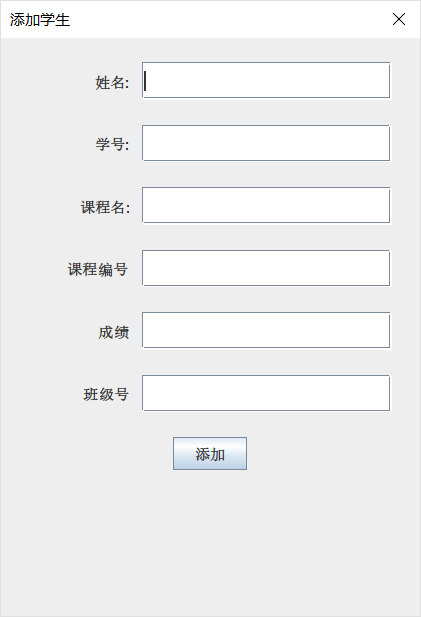
\includegraphics[width = 0.8\textwidth]{../pic/3/3.4.png}
    \caption{添加界面}

\end{figure}\begin{figure}[H]
    \centering
    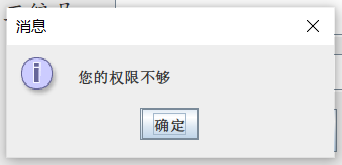
\includegraphics[width = 0.5\textwidth]{../pic/3/3.5.png}
    \caption{违权界面}
\end{figure}



\subsection{Action事件和RBAC权限管理相联系}
下面要做的就是将主界面的这些button添加rbac模型权限的ActionListener



\begin{lstlisting}[language = Java,
    caption = {AddPermissionPanel.java L50-69}]

// 为按钮设置监听器
actionButton.addActionListener(new AbstractAction() {
    @Override
    public void actionPerformed(ActionEvent e) {
        try {
            Statement statement = connection.createStatement();
            Map<String, String> map = new HashMap<>();
            map.put("action_id", MysqlUtil.getNextId("t_action", "action_id"));
            map.put("action_name", actionText.getText());
            // 将该操作添加到数据库中
            String insertObj = MysqlUtil.Insert("t_action", map);
            statement.executeUpdate(insertObj);

            //返回结果
            new ResultDialog("Success!");

        } catch (SQLException ex) {
            ex.printStackTrace();
        }
    }
});

\end{lstlisting}


\begin{lstlisting}[
    language = Java,
    caption = {MainPanel.java L132-150}]

// 获取当前用户的 权限并disable菜单栏的对应按钮
try {
    Statement statement = connection.createStatement();
    String getPermissionSql = "select permission_name from t_user_info,t_permission,t_role_permission where info_id=" + info_id + " and t_user_info.role_id=t_role_permission.role_id and t_role_permission.permission_id=t_permission.permission_id";
    ResultSet rs = statement.executeQuery(getPermissionSql);
    Set<String> permissionSet = new HashSet<>();
    while (rs.next()) {
        permissionSet.add(rs.getString(1));
    }
    System.out.println(permissionSet.toString());
    // 禁用该用户没有的权限
    for (MyMenuItem menuItem : itemList) {
        if (!permissionSet.contains(menuItem.getPermission())) {
            menuItem.setEnabled(false);
        }
    }
} catch (SQLException e) {
    e.printStackTrace();
}

\end{lstlisting}

\begin{lstlisting}[
    language = Java,
    caption = {PermissionManagePanel.java L196-270}
]

public void setMakePermissionTable() {

    makePermissionTable.removeAll();

    // 获取所有操作对象列表
    Obj[] objList = getObj();

    // 获取所有操作动作列表
    Action[] actionList = getAction();

    // 获取已经分配好的所有权限
    Permission[] permissionList = getPermission();

    // 为设置表格设置样式
    makePermissionTable.setLayout(new GridLayout(0, objList.length + 1, 10, 3));
    makePermissionTable.setBounds(20, 110, 700, (actionList.length + 1) * 30);

    // 第一行为所有的操作对象
    makePermissionTable.add(new JLabel()); //占位
    for (Obj obj : objList) {
        makePermissionTable.add(new JLabel(obj.objName));
    }

    // 初始化选择框并添加监听对象,在监听到勾选状态发生改变时上传数据到数据库
    checkBoxes = new JCheckBox[actionList.length][objList.length];
    for (int i = 0; i < actionList.length; i++) {
        makePermissionTable.add(new JLabel(actionList[i].actionName));
        for (int j = 0; j < checkBoxes[i].length; j++) {
            checkBoxes[i][j] = new JCheckBox();
            makePermissionTable.add(checkBoxes[i][j]);
            Obj obj = objList[j];
            Action action = actionList[i];
            JCheckBox checkBox = checkBoxes[i][j];
            checkBox.addActionListener(new AbstractAction() {
                @Override
                public void actionPerformed(ActionEvent e) {
                    String objId = obj.objId;
                    String objName = obj.objName;
                    String actionId = action.actionId;
                    String actionName = action.actionName;
                    try {
                        Statement statement = connection.createStatement();
                        String changePermissionSql;
                        Map<String, String> map = new HashMap<>();
                        map.clear();
                        map.put("obj_id", objId);
                        map.put("action_id", actionId);

                        if (checkBox.isSelected()) {
                            // 新增对应的权限
                            String permission_id = MysqlUtil.getNextId("t_permission", "permission_id");
                            map.put("permission_id", permission_id);
                            map.put("permission_name", actionName + objName);
                            changePermissionSql = MysqlUtil.Insert("t_permission", map);
                        } else {
                            // 删除对应的权限
                            changePermissionSql = MysqlUtil.Delete("t_permission", map);
                        }
                        statement.executeUpdate(changePermissionSql);

                    } catch (SQLException ex) {
                        ex.printStackTrace();
                    }

                    System.out.println(actionName + objName);
                }
            });
        }
    }

    // 设置默认选中的权限组合
    for (Permission permission : permissionList) {
        checkBoxes[Integer.parseInt(permission.actionId) - 1][Integer.parseInt(permission.objId) - 1].setSelected(true);
    }
}    
\end{lstlisting}

\section{RBAC模型簇的分析与比较}

\begin{itemize}
    \item RBAC0模型:最基础最简单的RBAC思想
    \item RBAC1模型:基于RBAC0模型,增加了子角色,引入了继承概念,即子角色可以继承父角色的所有权限
    \item RBAC2模型:基于RBAC0模型,增加了对角色的一些限制:
    \begin{itemize}
        \item 角色互斥:同一用户不能分配到一组互斥角色集合中的多个角色,互斥角色是指权限互相制约的两个角色。
        \item 基数约束:一个角色被分配的用户数量受限。
        \item 先决条件角色:指要想获得较高的权限,要首先拥有低一级的权限。
        \item 运行时互斥:例如,允许一个用户具有两个角色的成员资格,但在运行中不可同时激活这两个角色。
    \end{itemize}
    \item RBAC3模型:综合了RBAC0、RBAC1和RBAC2的所有特点。
\end{itemize}

\begin{table}[H]
    \centering
    \begin{tabular}{|l|c|c|}
        \hline
            & 特点               & 适用场景               \\ \hline
        RBAC0 & 最基础              & 普通无限制场景            \\ \hline
        RBAC1 & RBAC0 + 继承(等级)   & 层级分明的管理人员权限分配      \\ \hline
        RBAC2 & RBAC0 + 约束(职责分离) & 存在互斥的职位            \\ \hline
        RBAC3 & RBAC1 + RBAC2    & 同时符合RBAC1和RBAC2的场景 \\ \hline
    \end{tabular}
\end{table}

\section{总结与回顾}

本题目可以说是本学期开学以来所有科目中对我挑战性最大的一个题目,因为我并没有java GUI、DBAC、mysql和
PowerDesigner的操作基础,可以说除了RBAC的理论知识完全零基础。

在我写代码的过程中PowerDesigner的工具套件对我帮助最大,概念模型转物理模型再转sql源码的功能
大大加快了我的进度。


\end{document}